% use the answers clause to get answers to print; otherwise leave it out.
\documentclass[11pt,answers,addpoints]{exam}
%\documentclass[11pt,addpoints]{exam}
\RequirePackage{amssymb, amsfonts, amsmath, latexsym, verbatim, xspace, setspace}
\usepackage{graphicx}

% By default LaTeX uses large margins.  This doesn't work well on exams; problems
% end up in the "middle" of the page, reducing the amount of space for students
% to work on them.
\usepackage[margin=1in]{geometry}
\usepackage{enumerate}
\usepackage[hidelinks]{hyperref}

% Here's where you edit the Class, Exam, Date, etc.
\newcommand{\class}{NPRE 555}
\newcommand{\term}{Fall 2025}
\newcommand{\assignment}{HW 7}
\newcommand{\duedate}{2025.10.20}
%\newcommand{\timelimit}{50 Minutes}

\newcommand{\nth}{n\ensuremath{^{\text{th}}} }
\newcommand{\ve}[1]{\ensuremath{\mathbf{#1}}}
\newcommand{\Macro}{\ensuremath{\Sigma}}
\newcommand{\vOmega}{\ensuremath{\hat{\Omega}}}

% For an exam, single spacing is most appropriate
\singlespacing
% \onehalfspacing
% \doublespacing

% For an exam, we generally want to turn off paragraph indentation
\parindent 0ex

%\unframedsolutions

\begin{document} 

% These commands set up the running header on the top of the exam pages
\pagestyle{head}
\firstpageheader{}{}{}
\runningheader{\class}{\assignment\ - Page \thepage\ of \numpages}{Due \duedate}
\runningheadrule

\class \hfill \term \\
\assignment \hfill Due \duedate\\
\rule[1ex]{\textwidth}{.1pt}
%\hrulefill

%%%%%%%%%%%%%%%%%%%%%%%%%%%%%%%%%%%%%%%%%%%%%%%%%%%%%%%%%%%%%%%%%%%%%%%%%%%%%%%%%%%%%
%%%%%%%%%%%%%%%%%%%%%%%%%%%%%%%%%%%%%%%%%%%%%%%%%%%%%%%%%%%%%%%%%%%%%%%%%%%%%%%%%%%%%
\begin{itemize}
        \item Show your work.
        \item This work must be submitted online as a \texttt{.pdf} through Canvas.
        \item Work that appears to have been handwritten with a dull pencil or
                photographed with a potato will not be graded generously.
                Typset your homework if possible. Write and digitize carefully if not.
        \item Work completed with LaTeX earns 1 extra point. Submit
                source file (\texttt{.tex}) along with
                the \texttt{.pdf} file.
        \item If this work is completed with the aid of a numerical program
                (such as Python, Wolfram Alpha, or MATLAB) all scripts and data
                must be submitted in addition to the \texttt{.pdf}.
        \item If you work with anyone else, document what you worked on together.
\end{itemize}
\rule[1ex]{\textwidth}{.1pt}

% ---------------------------------------------
\begin{questions}

        % ---------------------------------------------
        \question[20] Write the one-dimensional, one-speed, steady-state $S_2$ 
        equations with an isotropic source and isotropic scattering.
        \begin{solution}
                solution here
        \end{solution}

        % ---------------------------------------------
        \question[20] Prove that the $S_2$ and $P_1$ equations are equivalent 
        for a steady state, single speed problem with isotropic source and 
        scattering.
        \begin{solution}
                solution here
        \end{solution}

        % ---------------------------------------------
        \question[10] Why are odd order $S_N$ equations avoided?
        \begin{solution}
                solution here
        \end{solution}

        % ---------------------------------------------
        \question 
        Consider the infinite slab with two regions in Figure \ref{fig:slab}. 
        There  are vacuum boundary conditions on both sides of the slab. 
        Scattering is isotropic in the lab system.

        In region 1:
        \begin{itemize}
                \item Width is $2cm$.
                \item $\Sigma_t = \frac{1}{cm}$.
                \item $\Sigma_a = \frac{0.5}{cm}$.
                \item There is a uniformly distributed isotropic unit source $\left(1\left[\frac{n}{cm}\right]\right)$.
        \end{itemize}

        In region 2:
        \begin{itemize}
                \item Width is $4cm$.
                \item $\Sigma_t = \frac{1.5}{cm}$.
                \item $\Sigma_a = \frac{1.2}{cm}$.
                \item There is no source.
        \end{itemize}

        \begin{figure}[htb!]
                \begin{center}
                        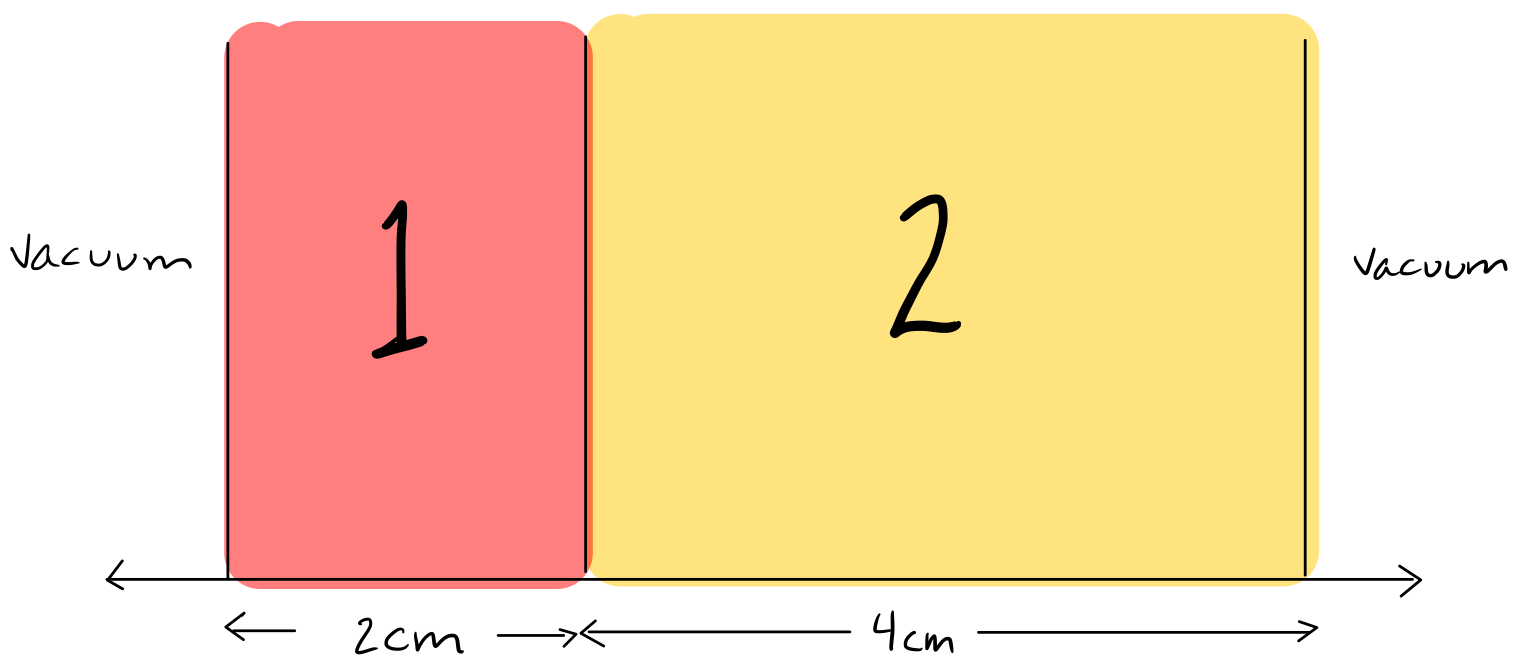
\includegraphics[width=0.5\textwidth]{slab-prob.png}
                \end{center}
                \caption{Infinite slab with two regions.}
                \label{fig:slab}
        \end{figure}


        \begin{parts}
                \part[40] Use Gauss-Legendre quadrature to solve the $S_N$ equations 
        for the slab problem below using a diamond difference approach. 


        \begin{solution}
                solution here
        \end{solution}
        
        \part[10] Refine your solution to part c by refinding the spatial mesh of your solution and angular quadrature until the scalar flux asymptotically converges.
        What is the spatial order of convergence of the method?
        \begin{solution}
                solution here
        \end{solution}
        \end{parts}


\end{questions}



%\bibliographystyle{plain}
%\bibliography{hw01}
\end{document}
